\documentclass{standalone}
\usepackage[dvipsnames]{xcolor}
\usepackage[skins]{tcolorbox}

\usepackage{tikz}
\usetikzlibrary{calc}
\usetikzlibrary{shapes}
\usetikzlibrary{decorations.pathmorphing}
\tikzset{snake it/.style={decorate, decoration={snake,  amplitude=0.33pt}}}

\usepackage{fontspec}
\begin{document}

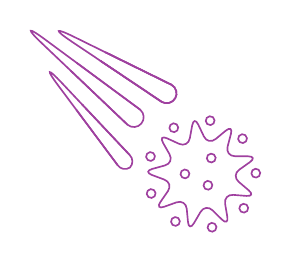
\begin{tikzpicture}%[every path/.style={violet!75}]
\clip(-2.21,-0.77) rectangle (0.78,1.86);

%\begin{scope}[rotate=-40, scale=0.25, every path/.style={ultra thick, black}]
%\node (A) at (5:3cm) {};
%\node (B) at (27.5:1.5cm) {};
%\node (C) at (-4, 2.5) {};
%\node (D) at (-4,1.5) {};
%\node (E) at (-11.5,2) {};
%
%
%\node[draw, star, star points = 9, star point ratio = 0.5, rounded corners=1.25mm, minimum size=3.0cm, rotate=27.5, transform shape] (a) at (0,0) {};
%
%%	\node[draw, circle, semithick, minimum size=1.25cm, transform shape] at (219.25:0.5) {};
%	\node[draw, circle, minimum size=0.45cm, transform shape] at (219.25:0.85) {};
%		\node[draw, circle, minimum size=0.45cm, transform shape] at (99.25:0.95) {};
%		\node[draw, circle, minimum size=0.45cm, transform shape] at (339.25:0.65) {};
%
%	\foreach \i in {0,1,2,3,4,5,6,7,8}
%		\node[draw, circle, transform shape, minimum size=0.45cm] (a\i) at (40*\i + 1:2.75cm) {};
%
%
%% Tail
%    \path[draw,, bend right=45,  rotate around={10:(-4, 2)}] ($ (-4,1.5) !.5! (-11.5,2) $) -- (-4,1.5) to (-3.5, 2) to (-4, 2.5) -- ($ (-4,2.5) !.5! (-11.5,2) $);
%	\path[draw,, bend right=45,  rotate around={10:(-4, 2)}] ($ (-4,1.5) !.5! (-11.5,2) $) -- (-4,1.5) to (-3.5, 2) to (-4, 2.5) -- ($ (-4,2.5) !.5! (-11.5,2) $);
%	\path[draw, rounded corners=5mm, rotate around={10:(-4, 2)}] (-4, 2.5) to (-11.5,2) to  (-4,1.5);
%
%	\path[draw, bend right=45,  rotate around={0:(-4.5, 0)}] ($ (-4.5,-0.5) !.5! (-12.5,0) $) --(-4.5,-0.5) to (-4, 0) to (-4.5, 0.5) -- ($ (-4.5,0.5) !.5! (-12.5,0) $);
%	\path[draw, rounded corners=5mm, rotate around={0:(-4.5, 0)}] (-4.5, 0.5) to (-12.5,0) to  (-4.5,-0.5);
%	
%	\path[draw, bend right=45,  rotate around={-10:(-3.5, -2)}] ($ (-3.5,-2.4) !.5! (-10.5,-2) $) -- (-3.5,-2.4) to (-3, -2) to (-3.5, -1.6) -- ($ (-3.5,-1.6) !.5! (-10.5,-2) $);
%	\path[draw, rounded corners=5mm, rotate around={-10:(-3.5, -2)}] (-3.5, -1.6) to (-10.5,-2) to  (-3.5,-2.4);
%\end{scope}

\begin{scope}[rotate=-40, scale=0.25, every path/.style={semithick, violet!75}]
\node (A) at (5:3cm) {};
\node (B) at (27.5:1.5cm) {};
\node (C) at (-4, 2.5) {};
\node (D) at (-4,1.5) {};
\node (E) at (-11.5,2) {};


\node[draw, star, star points = 9, star point ratio = 0.5, rounded corners=1.25mm, minimum size=3.0cm, rotate=27.5, transform shape] (a) at (0,0) {};

%	\node[draw, circle, semithick, minimum size=1.25cm, transform shape] at (219.25:0.5) {};
	\node[draw, circle, minimum size=0.45cm, transform shape] at (219.25:0.85) {};
		\node[draw, circle, minimum size=0.45cm, transform shape] at (99.25:0.95) {};
		\node[draw, circle, minimum size=0.45cm, transform shape] at (339.25:0.65) {};

	\foreach \i in {0,1,2,3,4,5,6,7,8}
		\node[draw, circle, transform shape, minimum size=0.45cm] (a\i) at (40*\i + 1:2.75cm) {};


% Tail
    \path[draw,, bend right=45,  rotate around={10:(-4, 2)}] ($ (-4,1.5) !.5! (-11.5,2) $) -- (-4,1.5) to (-3.5, 2) to (-4, 2.5) -- ($ (-4,2.5) !.5! (-11.5,2) $);
	\path[draw,, bend right=45,  rotate around={10:(-4, 2)}] ($ (-4,1.5) !.5! (-11.5,2) $) -- (-4,1.5) to (-3.5, 2) to (-4, 2.5) -- ($ (-4,2.5) !.5! (-11.5,2) $);
	\path[draw, rounded corners=5mm, rotate around={10:(-4, 2)}] (-4, 2.5) to (-11.5,2) to  (-4,1.5);

	\path[draw, bend right=45,  rotate around={0:(-4.5, 0)}] ($ (-4.5,-0.5) !.5! (-12.5,0) $) --(-4.5,-0.5) to (-4, 0) to (-4.5, 0.5) -- ($ (-4.5,0.5) !.5! (-12.5,0) $);
	\path[draw, rounded corners=5mm, rotate around={0:(-4.5, 0)}] (-4.5, 0.5) to (-12.5,0) to  (-4.5,-0.5);
	
	\path[draw, bend right=45,  rotate around={-10:(-3.5, -2)}] ($ (-3.5,-2.4) !.5! (-10.5,-2) $) -- (-3.5,-2.4) to (-3, -2) to (-3.5, -1.6) -- ($ (-3.5,-1.6) !.5! (-10.5,-2) $);
	\path[draw, rounded corners=5mm, rotate around={-10:(-3.5, -2)}] (-3.5, -1.6) to (-10.5,-2) to  (-3.5,-2.4);
\end{scope}


%% Snakey Tail
%	\path[draw, semithick, bend right=45,  rotate around={10:(-4, 2)}] ($ (-4,1.5) !.025! (-10.25,2) $) -- (-4,1.5) to (-3.5, 2) to (-4, 2.5) -- ($ (-4,2.5) !.025! (-10.25,2) $);
%	\path[draw, semithick, rotate around={10:(-4, 2)}, snake it] ($ (-4,1.5) !.025! (-10.25,2) $) to (-10.25, 2);
%	\path[draw, semithick, rotate around={10:(-4, 2)}, snake it] ($ (-4,2.5) !.025! (-10.25,2) $) to (-10.25,2);
%
%	\path[draw, semithick, bend right=45,  rotate around={0:(-4.5, 0)}] ($ (-4.5,-0.5) !.025! (-12.5,0) $) --(-4.5,-0.5) to (-4, 0) to (-4.5, 0.5) -- ($ (-4.5,0.5) !.025! (-12.5,0) $);
%	\path[draw, semithick, snake it] ($ (-4.5,0.5) !.025! (-12.5,0) $) to (-11.25,0);
%		\path[draw, semithick, snake it] ($ (-4.5,-0.5) !.025! (-12.5,0) $) to (-11.25,0);
%
%	\path[draw, semithick, bend right=45,  rotate around={-10:(-3.5, -2)}] ($ (-3.5,-2.4) !.025! (-9.5,-2) $) -- (-3.5,-2.4) to (-3, -2) to (-3.5, -1.6) -- ($ (-3.5,-1.6) !.025! (-9.5,-2) $);
%	\path[draw, semithick, rotate around={-10:(-3.5, -2)}, snake it] ($ (-3.5,-2.4) !.025! (-9.5,-2) $) to (-9.5,-2);
%	\path[draw, semithick, rotate around={-10:(-3.5, -2)}, snake it] ($ (-3.5,-1.6) !.025! (-9.5,-2) $) to (-9.5,-2);

%\end{scope}

\end{tikzpicture}
\end{document}
